
\section{Results and Discussion}
%\resultsTips % Delete when no longer needed
\subsection{Uniform random state preparation}

We first applied the proposed state preparation method
to prepare uniformly sampled quantum states. Exact state preparation approaches using UCG 
\cite{bergholm2005quantum}, alternating ansatz VQC (AA-VQC) \cite{zhang2020toward}, and 
ADAPT-VQE \cite{grimsley2019adaptive} were also validated for the random uniform quantum states. In our experiments using randomly generated states, we tested qubit numbers from 5
to 14, inclusive. For each qubit number, 100 quantum states were uniformly, and randomly
sampled. 
When determining the classical runtime, the number of CX gates in the AA-VQC was set 
to $2^{n-1}$. This number was chosen because each CX gate attaches four free 
parameters, therefore, approximately $2^{n-1}$ CX gates are necessary for the 
number of circuit parameters to exceed the number of free parameters in an 
$n$-qubit quantum state. Under these conditions, the VQC should be able to prepare
any arbitrary $n$-qubit quantum state with high fidelity.

To determine the number of CX gates needed for AA-VQC, we trained VQCs with varying 
numbers of layers and reported the CX gate count corresponding to the minimum number 
of layers needed to achieve an average fidelity of 0.95. However, this minimum CX 
count also depends on the number of gradient descent steps used to optimize the 
angles: more layers require less training. To ensure a sufficiently large but also 
fair number of training iterations for each $n$, we trained an AA-VQC with $2^{n-1}$ CX 
gates on the first three quantum states and recorded the number of training 
iterations required to achieve 0.95 fidelity on all three states. Then, the number of 
training iterations was set to twice the sum of those numbers. This ensured that the 
number of training iterations was approximately six times as many as actually 
necessary for that specific number of qubits, preventing insufficient training from 
marring the results. CX gate count experiments were not run for the UCG method. This is because the number 
of CX gates depends on whether the circuit transpiler finds good circuit 
optimizations for LNN. However, using the exact nature of this algorithm, it was 
determined that this method uses $2\times2^n+2n-19$ CX gates to prepare an n-qubit 
quantum state (proof given in the Appendix). 


\begin{figure}[h]
\centering
\includegraphics[width=0.95\linewidth]{main/figs/fig2.png}
\caption{a) Average classical runtime versus number of qubits for each QSP method,
plotted on a linear-log scale. Only the ISA and UCG methods were able to prepare
the quantum states for $n$ up to 14; the AA-VQC method timed out (more than 1 hour
to prepare 100 states) after $n = 9$ and the ADAPT-VQE method timed out after
$n=7$. b) Average number of CX gates used to prepare 100 randomly generated quantum states versus number of qubits. The values in the ISA and ADAPT-VQE column show two decimal digits, since the number of CX gates used varied across quantum states. By contrast, the values for the UCG column were theoretically determined.}
\label{fig2}
\end{figure}

\begin{figure}[h]
\centering
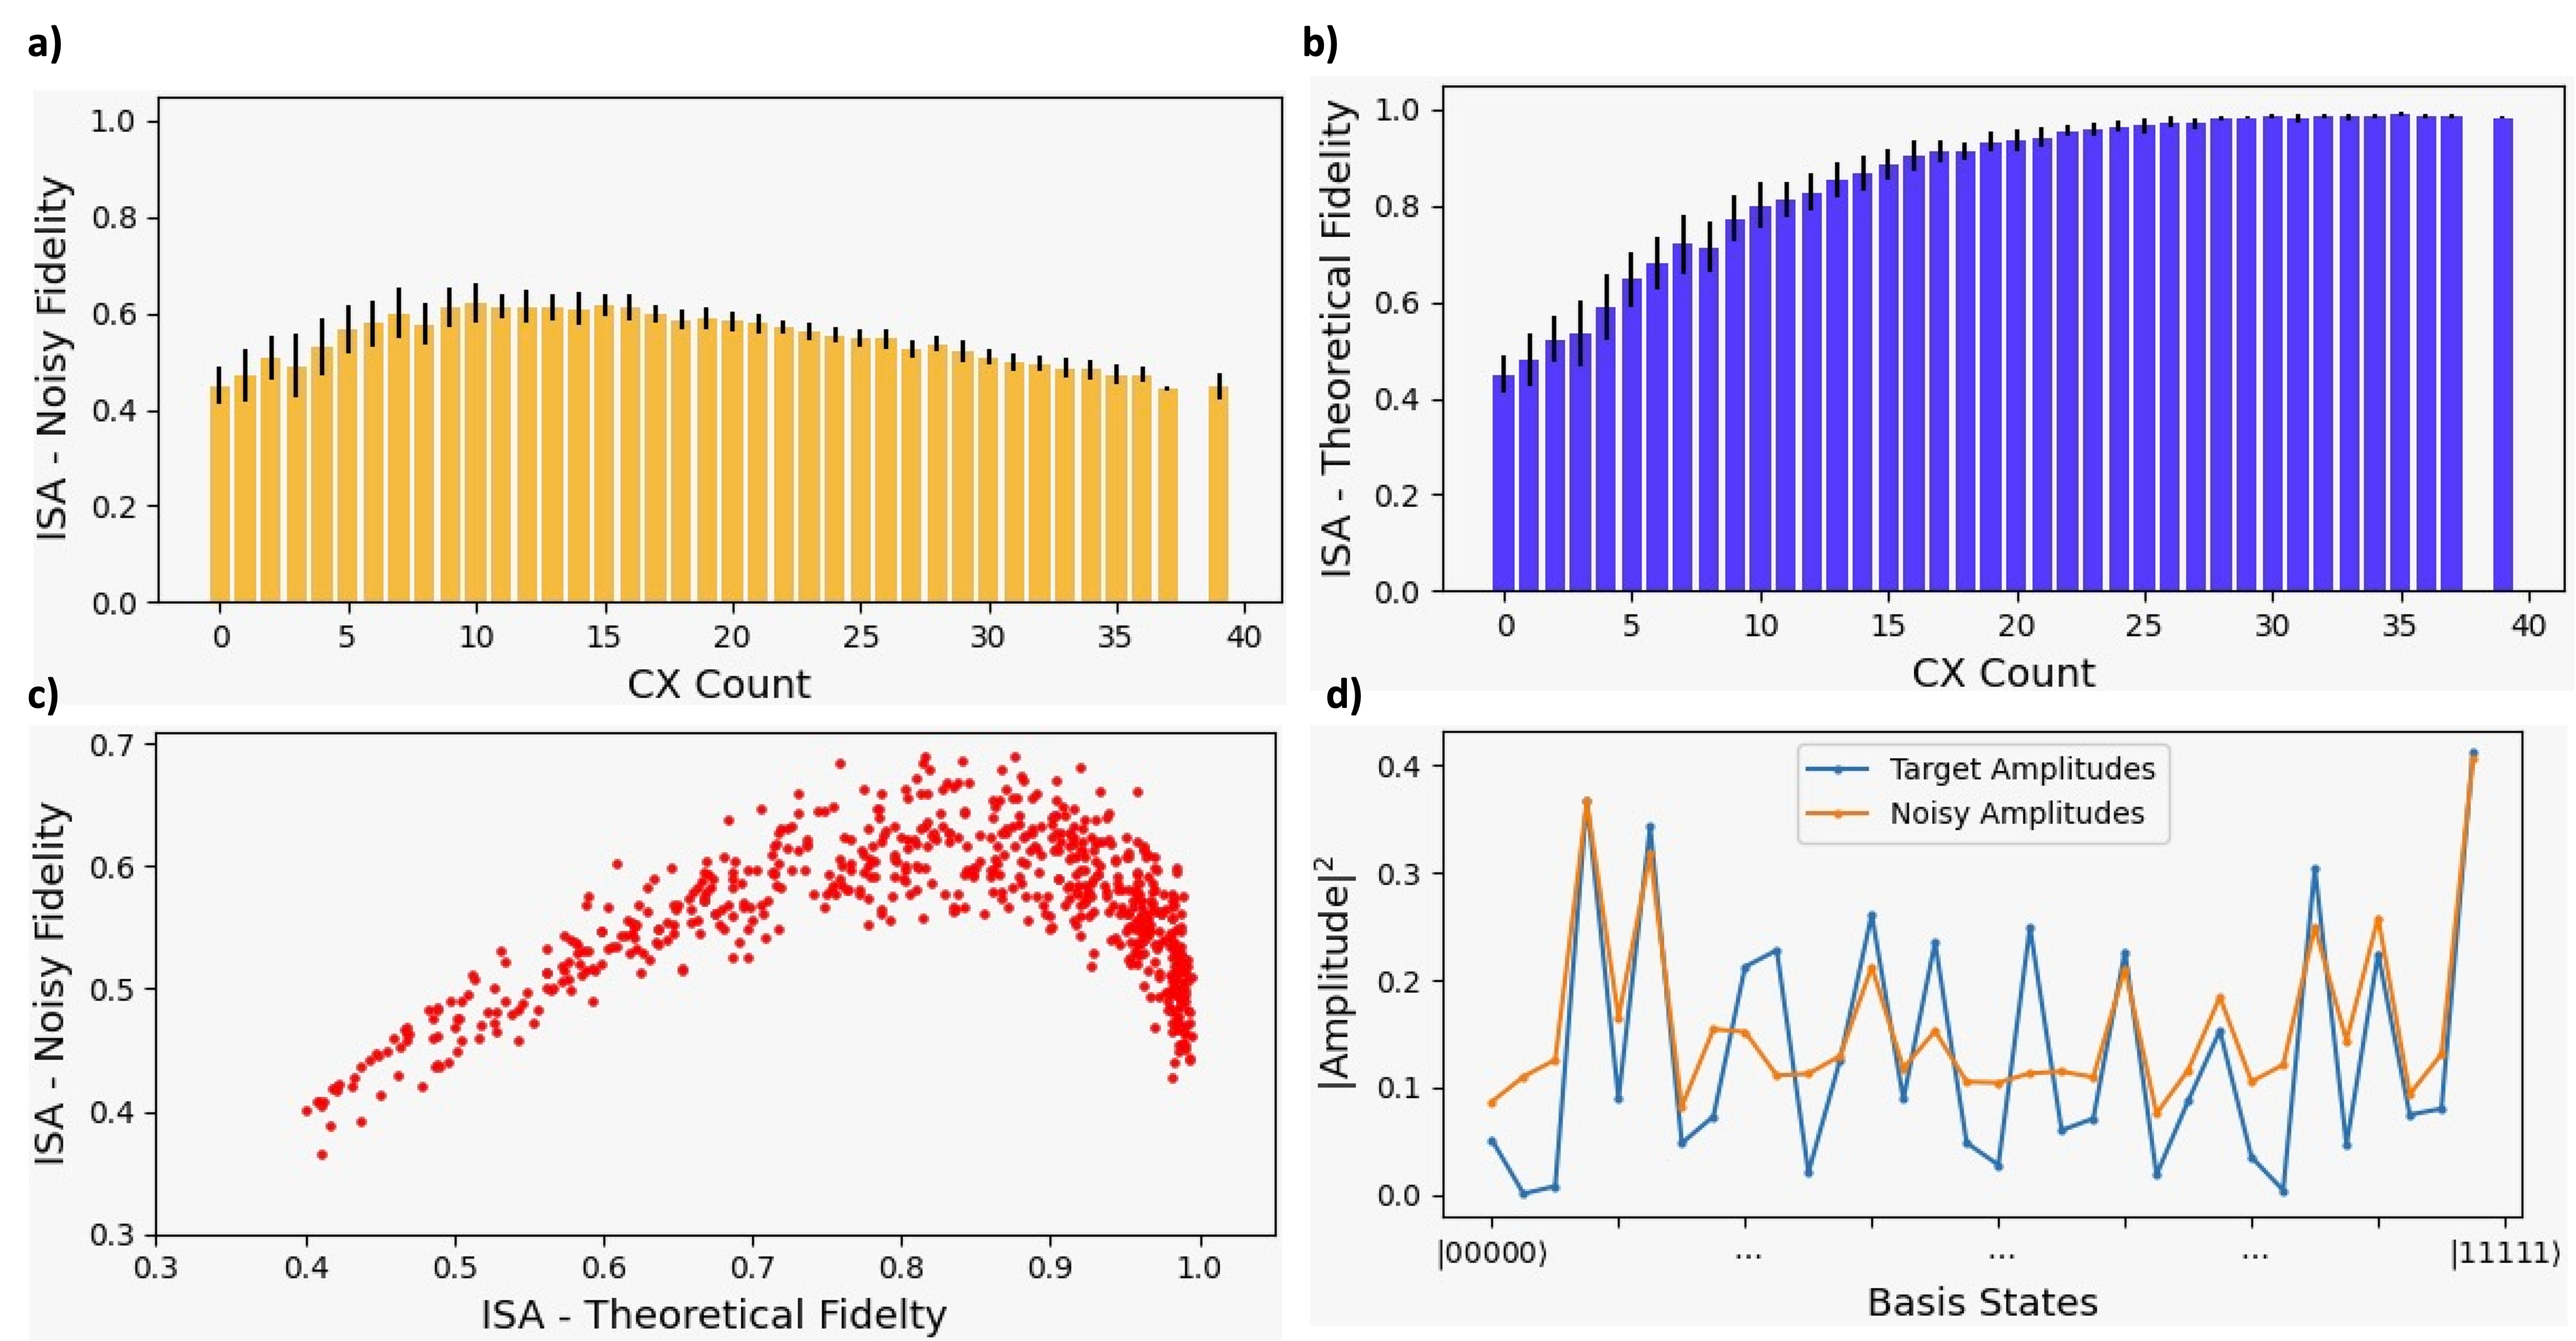
\includegraphics[width=0.95\linewidth]{main/figs/fig3.png}
\caption{Theoretical fidelity, noisy fidelity, and CX gate count for ISA on randomly
sampled five-qubit states on imbq\_melbourne quantum hardware. a)Noisy fidelity versus CX gate count across all 100 states. The error bars represent one
standard deviation at each CX gate count. The bar chart shows that the noisy fidelity
peaks around 10 CX gates. b) theoretical fidelity
versus CX gate count across all 100 states. The error bars represent one standard
deviation at each CX count. The graph shows that as CX gate count increases,
theoretical fidelity increases. c) Noisy fidelity
versus theoretical fidelity. The scatter plot shows that increasing theoretical fidelity
increases the noisy fidelity up to a theoretical fidelity of 0.8, then the curve
inverts and the two quantities become negatively correlated. d) Target state and prepared state amplitude vs basis
vector for the first randomly sampled quantum state. This figure compares the target quantum state
with the quantum state prepared on noisy hardware - while the peaks, corresponding
to large amplitudes, approximately match, the valleys corresponding to smaller 
amplitudes match less well.}
\label{fig3}
\end{figure}




\subsection{Fidelity of protein-encoded states}
For the second set of experiments, we sampled 20 proteins from the proteome of Homo 
sapiens from the UniProtKB database \cite{consortium2015uniprot}. We embedded these proteins into 
continuous, 1024-dimensional feature vectors using the ProtT5 pre-trained protein 
language model \cite{elnaggar2020prottrans}. We encoded these features into ten-qubit quantum states using 
real amplitude encoding. Classical runtime and CX gate counts were measured using the 
same methods as in the first set of experiments. Theoretical fidelities were also 
determined using the gate sequence outputs of each of the methods. For the third set of experiments, we prepared five-qubit quantum states on Qiskit’s
FakeMelbourneV2 machine, which features a LNN architecture on the first five qubits. 
We sampled 100 five-qubit states uniformly at random. For each state, we ran our ISA 
implementation with target fidelity thresholds ranging from 0.4 to 0.95 in increments 
of 0.05, then included an additional target fidelity threshold of 0.98, for a total 
of 13 trials per state. For each trial, the theoretical fidelity, noisy fidelity, and 
CX gate count were determined. Different target fidelity thresholds for the same 
state sometimes yielded identical gate sequences and corresponding fidelities; these 
duplicates were removed from our results. 

The AA-VQC method needed 71 layers to achieve a minimum average fidelity of 
0.95, corresponding to 320 CX gates. The fidelity of UCG is exactly  1.0, as 
it's an exact state preparation method rather than an approximation. Figure \ref{fig2}b
shows that the number of CX gates needed for the VQC-based methods is 
approximately $0.3N = 307.2$, which is consistent with the CX gate counts
reported for AA-VQC and ADAPT-VQE methods in Table 2. In addition, the CX gate
counts for ISA and UCG in Table 2 are consistent with those shown in Table 1.
Thus, all methods returned similar gate counts for both protein-encoded states
and randomly generated states. In addition, the classical runtimes shown in
Table 2 for UCG and ISA methods are consistent with those presented 
in Figure \ref{fig2}a. In addition, despite the timeout for the VQC-based methods at ten 
qubits, as shown in Figure \ref{fig2}, the classical runtime values are consistent with 
the general trend of pure VQC being several orders of magnitude slower than ISA 
and ADAPT-VQE being an order of magnitude slower than AA-VQC. Thus, the 
classical runtime results for protein-encoded states are consistent with those 
for general quantum states.

\begin{table}[h]
\centering
\caption{Average number of CX gates used to prepare 100 randomly generated quantum states versus number of qubits. The values in the ISA and ADAPT-VQE column show two decimal digits, since the number of CX gates used varied across quantum states. By contrast, the values for the UCG column were theoretically determined, and are therefore whole numbers. In addition, the values for AA-VQC were calculated by finding the minimum number of CX gates corresponding to an average fidelity of 0.95 - these are also whole numbers.}
\begin{tabular}{|c||c|c|c|c|}
\hline
Number of Qubits & ISA & UCG & ADAPT-VQE & AA-VQC\\
\hline
5 & 24.08 & 55 & 13.67 & 14 \\
6 & 60.98 & 121 & 25.97 & 28 \\
7 & 143.46 & 251 & 47.96 & 48 \\
8 & 319.02 & 509 & 88.76 & 91 \\
9 & 689.32 & 1023 & 164.22 & 180 \\
10 & 1439.6 & 2049 & TIMEOUT & TIMEOUT \\
11 & 2952.66 & 4099 & & \\
12 & 5991.51 & 8197 & & \\
13 & 12123.3 & 16391 & & \\
14 & 24538 & 32777 & & \\
\hline
\end{tabular}
\end{table}




\subsection{Computational performance}
Figure \ref{fig2}a shows the average classical runtime versus the number of qubits for each
method. For all numbers of qubits tested, the ISA implementation ran the fastest,
however, the ISA method's classical runtime increases faster with qubit number
compared to the UCG method. Thus, the UCG method is expected to be faster than ISA
for more than 14 qubits. Both methods were orders of magnitude faster than the
variational methods. This reflects the intense computational cost incurred by
the gate optimization procedures.

\begin{table}[h]
\centering
\caption{Minimum CX gate count and classical runtime to achieve 0.95 ideal
fidelity for each state preparation method. Each result is an average across 
the 20 trials of preparing distinct protein-encoded quantum states.}
\begin{tabular}{|c|c|c|}
\hline
Method & CX gate count & Classical Runtime \\
\hline
ISA & 1422.3 & $6.420 \times 10^{-2}$ \\
UCG & 2049 & $1.801 \times 10^0$ \\
ADAPT-VQE & 286.0 & $6.424 \times 10^3$ \\
AA-VQC & 320 & $4.895 \times 10^1$ \\
\hline
\end{tabular}
\end{table}

Table 1 shows the average number of CX gates used by each method as a function of the 
number of qubits. The UCG method uses the most CX gates. The ISA method uses somewhat 
fewer CX gates, while the variational methods use the fewest CX gates. The 
variational methods far outperform the non-variational methods in this regard, 
demonstrating the effectiveness of the variational optimization procedure. That said, 
the ISA method is shown to outperform the UCG method without any variational angle 
tuning procedure, indicating that ISA is able to find good QSP gate sequences.

The number of free parameters in the quantum circuit is proportional to the number of 
CX gates; the number of free parameters needed is proportional to $N$, the number of 
complex amplitudes in the target state. Therefore, we hypothesized that the number of 
CX gates would be approximately proportional to $N$ and try to determine the constant 
factor by graphing CX count divided by $N$ as a function of the number of qubits. If 
the CX count is indeed proportional to $N$, then the graph should approach a
horizontal line for large $n$, asymptotically approaching the constant factor. 
Figure \ref{fig2}b shows the average number of CX gates divided by $N$ as a function of 
qubit number for each method. For our ISA implementation, the curve increases for 
$n < 10$, then stabilizes to around 1.5. Thus, we conclude that our ISA 
implementation uses approximately $1.5N$ CX gates for randomly sampled quantum states.
By contrast, the UCG method is shown to use $2N + 2n - 19$ CX gates, which is $2N$ to
the leading order. Thus, the ISA method is shown to use approximately 25\% fewer CX gates
compared to the UCG method. However, both variational methods stabilize to around
0.3, which is about 5 times better than our ISA implementation, demonstrating the
effectiveness of the (computationally expensive) gate optimization procedure.


\subsection{Simulations with noisy quantum circuits}
Figure \ref{fig3} depicts the theoretical fidelity, noisy fidelity, and CX
gate count from the third set of experiments. Figure
\ref{fig3} shows that as the theoretical fidelity
increases from 0.4 to 0.8, the noisy fidelity increases from 0.4 to 0.6. 
Further increases in theoretical fidelity, however, cause the noisy fidelity 
to decrease. This inverse-U shaped correlation between the noisy fidelity and 
the theoretical fidelity is expected because increasing target fidelity 
increases the CX gate count; at first, CX gates improve the quality of the 
prepared state, but beyond a point, the marginal utility of a CX gate 
is outweighed by the noise it introduces. Indeed, Figures 
\ref{fig3}a and \ref{fig3}b corroborate these
expectations; while increasing CX gate count monotonically
increases theoretical fidelity, an increase in CX gate count improves noisy
fidelity only up to a peak of 0.68, around 10 CX gates. Figure 
\ref{fig3}d shows that the largest amplitudes in the prepared 
states match the largest amplitudes in the target state, but the smaller
amplitudes match less well. This is a direct consequence of how our 
ISA implementation approximates the target state as the sum of its largest 
amplitudes, then applies corrections for the smaller amplitudes. These 
corrections cannot prepare the smaller amplitudes perfectly, leading to a 
negative correlation between target amplitude magnitude and how closely it 
matches the corresponding amplitude in the prepared state.

\subsection{Hardware considerations and challenges}
For both the random and protein-encoded quantum states, our implementation of the ISA 
framework uses fewer CX gates than exact state preparation methods without incurring 
the variational optimization costs associated with VQC-based methods. However, the 
VQC-based methods are able to prepare quantum states using much fewer CX gates 
compared to the ISA method, and the UCG method is expected to be faster than ISA for 
quantum states on more than 14 qubits. This trend is expected: the less computation 
time a method uses, the lower the quality of its output.

In practice, every CX gate applied introduces hardware noise into the computation. 
Therefore, the design of quantum circuits will require a careful balance between 
using enough CX gates to approximate the desired computation, while not using so many 
CX gates as to corrupt the computation with noise. The ISA framework lends itself to 
a simple method for finding this balance: if too many CX gates are present in the 
state preparation algorithm, delete the gates corresponding to the last ISA 
iteration; if insufficient CX gates are present, perform more sparse approximation 
iterations. This works because each iteration of sparse approximation monotonically 
increases the state preparation fidelity and each additional iteration provides 
diminishing returns on fidelity increase. This idea was demonstrated our noisy 
simulation experiments. Different target fidelity thresholds led to different numbers 
of CX gates, corresponding to a range of different observed preparation fidelities. 
Finding the optimal CX count was reduced to identifying the optimal target fidelity 
threshold along the theoretical versus noisy fidelity plot for that particular state. 
By contrast, creating such a CX gate count vs noisy fidelity curve for a simple VQC 
method would require re-training the quantum circuit at every CX count sampled; for 
large numbers of qubits, this would require many repetitions of the parameter 
optimization procedure, driving up its already-expensive computational cost.

In addition, different quantum hardwares have different qubit connectivity. The 
only hardware-dependent steps in our ISA implementation are enumerating the 
compatible patterns $\{p\}$ and computing $CX(p)$, both of which can be done by an 
analogous breadth first search procedure. Thus, our ISA implementation can be easily 
adapted to different hardware connectivities.
However, the ISA method does face several limitations. Most importantly, our 
implementation of ISA uses four or five times as many CX gates as the VQC-based 
methods. This may cause ISA-generated gate sequences to induce much more noise on 
near term quantum hardware compared to VQC-based methods. This problem may eventually 
be mitigated by future work discovering alternative, easy-to-prepare classes of 
quantum states for approximating dense quantum states, then adapting those 
discoveries towards an improved ISA implementation. In addition, it may be possible 
to incorporate some variational training alongside ISA. However, the cost function, 
training schedule, gradient conditioning, and other things would need to be carefully 
designed to ensure such a hybrid method does not become a worse version of ADAPT-VQE 
or AA-VQC. Another limitation of the ISA method is that it cannot prepare quantum states that 
require extremely high fidelity. This is because the ISA method treats the dense 
target state as a sparse approximate state, therefore, some percentage of the 
fidelity will be lost on every sparse approximation, and chasing down these lost 
details would require many, many more iterations of ISA. That said, many applications 
of QSP, such as machine learning and sampling from probability distributions, require 
only approximate QSP.

